%===================================================================================
% JORNADA CIENTÍFICA ESTUDIANTIL 2013 - MATCOM, UH
%===================================================================================
% Esta plantilla ha sido diseñada para ser usada en los artículos de la
% Jornada Científica Estudiantil, MatCom 2015.
%
% Por favor, siga las instrucciones de esta plantilla y rellene en las secciones
% correspondientes.
%
% NOTA: Necesitará el archivo 'jcematcom.sty' en la misma carpeta donde esté este
%       archivo para poder utilizar esta plantila.
%===================================================================================



%===================================================================================
% PREÁMBULO
%-----------------------------------------------------------------------------------
\documentclass[a4paper,12pt,twocolumn]{article}

%===================================================================================
% Paquetes
%-----------------------------------------------------------------------------------
\usepackage{amsmath}
\usepackage{amsfonts}
\usepackage{amssymb}
\usepackage{jcematcom}
\usepackage[utf8]{inputenc}
\usepackage{listings}
\usepackage[pdftex]{hyperref}
%-----------------------------------------------------------------------------------
% Configuración
%-----------------------------------------------------------------------------------
\hypersetup{colorlinks,%
	    citecolor=black,%
	    filecolor=black,%
	    linkcolor=black,%
	    urlcolor=blue}

%===================================================================================



%===================================================================================
% Presentacion
%-----------------------------------------------------------------------------------
% Título
%-----------------------------------------------------------------------------------
\title{Problema 4: President's Path}

%-----------------------------------------------------------------------------------
% Autores
%-----------------------------------------------------------------------------------
\author{\\
\name Rodrigo García Gómez\email \href{mailto:rodrigo.garcia@estudiantes.matcom.uh.cu}{rodrigo.garcia@estudiantes.matcom.uh.cu}
}

%-----------------------------------------------------------------------------------
% Tutores
%-----------------------------------------------------------------------------------
\tutors{\\
Alfredo Somoza \emph{} \\
}

%-----------------------------------------------------------------------------------
% Headings
%-----------------------------------------------------------------------------------


%-----------------------------------------------------------------------------------
\ShortHeadings{}{Autores}
%===================================================================================



%===================================================================================
% DOCUMENTO
%-----------------------------------------------------------------------------------
\begin{document}

%-----------------------------------------------------------------------------------
% NO BORRAR ESTA LINEA!
%-----------------------------------------------------------------------------------

%-----------------------------------------------------------------------------------
\twocolumn[
\maketitle

%===================================================================================
% Resumen y Abstract
%-----------------------------------------------------------------------------------
\selectlanguage{spanish} % Para producir el documento en Español

%-----------------------------------------------------------------------------------
% Resumen en Español
%-----------------------------------------------------------------------------------
\begin{abstract}
Se debe calcular, para cada par de vértices, la cantidad de aristas que participan en algún camino de costo mínimo entre ellos. Como es usual, se implementará primero un algoritmo de “fuerza bruta” que probará todos los caminos entre todos los pares de vértices y almacenará en una lista (sin repetir) las aristas que participen en los caminos que tengan costo mínimo. Esto tendrá costo exponencial. $A$ continuación se implementa un algoritmo optimizado de la fuerza bruta que, a pesar de seguir teniendo un costo exponencial, resulta bastante más eficiente, pues evita el análisis de las aristas que no pertenecen a algún camino de costo mínimo entre los vértices siendo analizados. Gracias a la existencia de esta optimización, el proceso de testeo se vuelve más eficiente, al abrir la posibilidad de analizar casos con n y m de mayor tamaño.\\
Finalmente se llega a la implementación de un algoritmo considerablemente óptimo que realiza tres ciclos de $n^3$ iteraciones. Este se basa en la idea de calcular, para cada par de vértices $s$, $t$, y para cada vértice $v$ que participa en alguno de los caminos de menor costo entre $s$ y $t$, la cantidad de aristas que van hacia $v$, que participen en alguno de los caminos de menor costo entre $s$ y $v$.\\
\end{abstract}

%-----------------------------------------------------------------------------------
% English Abstract
%-----------------------------------------------------------------------------------
\vspace{0.5cm}



%-----------------------------------------------------------------------------------
% Palabras clave
%-----------------------------------------------------------------------------------


%-----------------------------------------------------------------------------------
% Temas
%-----------------------------------------------------------------------------------



%-----------------------------------------------------------------------------------
% NO BORRAR ESTAS LINEAS!
%-----------------------------------------------------------------------------------
\vspace{0.8cm}
]
%-----------------------------------------------------------------------------------


%===================================================================================

%===================================================================================
% Introducción
%-----------------------------------------------------------------------------------
\section{Texto del problema}
Good old Berland has $n$ cities and m roads. Each road connects a pair of distinct cities and is bidirectional. Between any pair of cities, there is at most one road. For each road, we know its length.\\

We also know that the President will soon ride along the Berland roads from city s to city $t$. Naturally, he will choose one of the shortest paths from $s$ to $t$, but nobody can say for sure which path he will choose.\\

The Minister for Transport is really afraid that the President might get upset by the state of the roads in the country. That is the reason he is planning to repair the roads in the possible President's path.\\

Making the budget for such an event is not an easy task. For all possible distinct pairs $s, t$ ($s<t$) find the number of roads that lie on at least one shortest path from $s$ to $t$.

\section{El problema}\label{sec:intro}
	
	Se tiene un grafo $G$ no dirigido de $n$ vértices y $m$ aristas. Se debe calcular para cada par de vértices $s$, $t$, la cantidad de aristas que pueden pertenecer a al menos uno de los caminos de costo mínimo entre ellos\\  
	
	Se da como entrada $n$, que representa la cantidad de vértices, $m$ que representa la cantidad de aristas y $m$ tuplas $u$, $v$, $l$, siendo $u$ y $v$ dos vértices conectados por una arista y $l$ el costo de esta. La salida debe ser una secuencia de enteros $c_{12}, c_{13}, … , c_{1n}, c_{23}, c_{24}, … , c_{2n}, … , c_{(n-1)n}$, siendo $c_{st}$ la cantidad de carreteras que pertenecen a algún camino más corto entre $s$ y $t$. La salida debe darse en el orden especificado y si algún par de vértices no tiene carreteras que lo conecte, el valor devuelto será 0.\\
  
   

%===================================================================================



%===================================================================================
% Desarrollo
%-----------------------------------------------------------------------------------
 
	\section{Algoritmo Floyd-Warshall}
		Para cada uno de los siguientes algoritmos, es utilizado el algoritmo de \texttt{\ttfamily floyd-Warshall} para calcular el camino mínimo entre cada uno de los vértices del grafo. El resultado de esto se almacena en la lista de nombre \texttt{\ttfamily distances}
	
	\begin{description}
		\item[Descripción:] Mediante este algoritmo se construirá una matriz distances, que en la posición u, v  tendrá la distancia de un camino mínimo de $u$ a $v$. La matriz se iniciará con \texttt{\ttfamily sys.maxsize} en todas las posiciones, excepto aquellas que representan a la distancia entre dos vértices adyacentes, en las que se pondrá el costo de la arista que los une. Luego se hará un ciclo por cada uno de los vértices $i$ de $G$ y, para cada pareja de vértices $u$, $v$, se verificará si la distancia hasta ahora calculada de $u$ a $i$, más la de $i$ a $v$ es menor que la de $u$ a $v$ (En otras palabras, si es mejor la forma actual de llegar de $u$ a $v$, o si es mejor llegar de $u$ a $i$, para entonces ir de $i$ a $v$ ). En caso de serlo, se actualiza el valor de distances en u, $v$.\\
		
	\end{description}
	
	
	\begin{description}
		\item[Demostración] Se demostrará que al finalizar la ejecución de \texttt{\ttfamily Floyd-Warshall}, en la matriz distances quedarán los valores de los caminos mínimos entre cada par de vértices $u,v$.\\
		
		Se define $d_i(u, v)$ como la matriz distances calculada por el algoritmo en la iteración i, o sea procesando al vértice i. se tiene que $p_i(u,v) = $ \texttt{\ttfamily min($p_{i-1}(u,v)$, $p_{i-1}(u, i)$}$ + p_{i-1}(i, v)$.\\
		
		Se demostrará por inducción en $i$ que si se cumple para $i$ la siguiente condición, también se cumplirá para $i+1$:\\
		Para la iteración i, $p_i(u, v) = cst$ tiene el costo de un camino de costo mínimo $C$ de $u$ a $v$ conteniendo como vértices interiores sólo a vértices que pertenecen a {$0, 1, ..., i$}\\
		$$i = 0$$
		En la primera iteración el único vértice interior sería 0, por tanto el costo mínimo de $u$ a $v$ conteniendo como nodos interiores sólo a vértices que pertenecen a {$0$} puede ser $cost(<u, v>)$ o $cost(<u, 0>) + cost(<0,v>)$ y $p_i(u, v)$ tendrá al menor de estos valores.
		$$i \Rightarrow i ¡ 1$$
		$C$ puede o no contener a $i$. Si no contiene a $i$ entonces es el mismo camino encontrado en la iteración $-1$. Si contiene a i, entonces, sean $C_1$ y $C_2$ los subcaminos de $C$ tales que van de $u$ a $i$ y de $i$ a $v$ respectivamente, note que tienen como vértices intermedios sólo a vértices de {$0, 1, ..., i-1$} y por tanto ambos fueron encontrados en la iteración $i-1$. Como $p_i(u, v)$ será igual a alguna de estas dos opciones, queda demostrado el paso inductivo.\\\\
		
		
		Al finalizar el algoritmo con la última iteración $i$, $p_i(u, v)$ tendrá el costo del camino mínimo de $u$ a $v$ tal que sus nodos internos pertenecen al conjunto de todos los vértices del grafo.		
	\end{description}	
	\begin{description}
		\item [Complejidad Temporal:] El algoritmo está conformado por tres ciclos anidados de $n$ iteraciones. Es fácil notar que su complejidad temporal es $O(n^3)$.
	\end{description}
	
	\section{Idea de Fuerza Bruta}

		Para cada pareja distinta de nodos $u$, $v$ se creará una lista (\texttt{\ttfamily walked}) que se rellenará con las carreteras caminadas (siempre que estas sean parte de algún camino de costo mínimo) mediante la funcion recursiva \texttt{\ttfamily calculate}, la cual estará simulando recorrer todos los caminos partiendo de $u$ y llegando a $v$. \\
		
		La funcion recibe la matriz vertices que para $i, j$ tiene valor 1 si existe carretera entre los vértices $i, j$ y 0 si no existe; la matriz \texttt{\ttfamily edges} que posee las distancias entre los vértices $i, j$; el vértice actual sobre el que se está parado; el vértice destino; la distancia que hay entre el vértice inical y final, y la lista \texttt{\ttfamily walked} que se quiere rellenar.\\
		
		Se llevará constancia de los vértices ya analizados mediante una lista \texttt{\ttfamily visited} que se irá llenando a medida que se camina sobre un vértice. Además se llevará constancia del costo del camino recorrido hasta cada momento. En cada llamado recursivo se analizará cada vértice v que posea una arista que lo conecte con el nodo actual siendo analizado (en la primera iteración este será el inicio del camino) y en caso de que v no haya sido visitado aún, se visitará mediante un llamado recursivo al algoritmo tomando a este como el vértice actual y con el costo del recorrido actual incrementado en el peso de la arista. Además, dicha arista será agregada a una lista \texttt{\ttfamily local\_walked} que almacena las aristas recorridas en el camino actual.\\
		
		Cuando el vértice actual y el destino sean el mismo, se habrá alcanzado el caso base, entonces se analiza si el costo recorrido hasta el momento es igual al la distancia mínima que se entra como parámetro. En caso negativo se retorna sin más pues el camino que se hizo no era de costo mínimo. En caso positivo sealmacena en \texttt{\ttfamily walked} todas las aristas que pertenezcan a \texttt{\ttfamily local\_walked} siempre que estas no estuvieran anteriormente y se retorna.\\
		
		Al finalizar la función, basta con agregar a la lista con los resultados para retornar, el tamaño de la lista \texttt{\ttfamily walked}. Los resultados tendrán el orden adecuado gracias a la forma en que está implementado el doble ciclo \texttt{\ttfamily for}.
		La correctitud del algoritmo está basada en el hecho de que se analizan todos los caminos posibles entre cada par de nodos, ya que se parte de uno, analizando todas sus aristas adyacentes y a partir de los nodos conectados con estas se repite el proceso hasta llegar a la arista destino.\\
		
		En cada llamado recursivo se ejecuta alguno de los dos ciclos \texttt{\ttfamily for} que a lo sumo tendrán una cantidad de iteraciones igual a la cantidad de aristas del grafo. Además la recursión analizará, para cada vértice, potencialmente todos los restantes vértices del grafo, para los que a su vez se realizará el mismo análisis. La función recursiva se llamará una cantidad cuadrática de veces (con respecto a n) en el doble ciclo \texttt{\ttfamily for} Por tanto la complejidad temporal del algoritmo será $n^2 * ((n + m)^n)$.\\
		
	\section{Optimización de la Fuerza Bruta}
	Se realiza una optimización del algoritmo anterior que, a pesar de no ser polinomial, es considerablemente más eficiente. La idea se basa en el hecho de que no es necesario hacer un llamado para analizar un vértice unido al actual, si la arista que los conecta no forma parte de ningún camino de costo mínimo entre el vértice inical y final. Para lograr esto se almacenará el valor que representa al vértice inical, además del que está siendo analizado actualmente y se tendrá acceso a la matriz \texttt{\ttfamily distances} que almacena las distancias mínimas entre todos los vértices. Luego, a la hora de decidir si desplazarse o no a un vértice v conectado con el actual, se analizará si la distancia mínima entre el vértice inical y el actual, más el peso de la arista que conecta al actual con v, más la distancia mínima entre $v$ y el nodo final es igual a la distancia mínima entre el nodo inical y final. En caso negativo, no será necesario analizar a $v$ por el camino actual en formación, puesto que de hacerlo, este no tendrá costo mínimo.\\
	
	Esta optimización previene la realización de muchas iteraciones innecesarias. De esta manera se puede utilizar el algoritmo con casos de prueba mayores en un menor tiempo y así permitir que el testeo a paritr de la comparación entre algoritmos sea más eficiente.\\
	
	\section{Algoritmo Óptimo}
	La idea es que, para cada par de nodos $init,dest$, la cantidad de aristas que participan en algún camino de costo mínimo que los una será igual a la suma de, para cada nodo $v$ que participa en alguno de los caminos de costo mínimo entre $init$ y $dest$, sus $inDegrees$. Esto es la cantidad de aristas adyacentes a v que participan en alguno de los caminos de costo mínimo de $init$ a $v$.\\
	
	 En la Figura 1 se ilustra un ejemplo del cálculo del $inDegree$ de un vértice. Note que $v$ forma parte de un camino de costo mínimo entre $init$ y $dest$ ($<init,a>, <a, v>, <v, dest>$) y hay dos aristas ($<a,v>$ y $<c,v>$) que son adyacentes a $v$ y forman parte de un camino de costo mínimo de $init$ a $v$ ($(<init, a>, <a,v>)$ y $(<init, c>, <c, v>)$ respectivamente). Por tanto el $inDegree$ de $v$ con respecto a $init$ y $dest$ tiene valor 2.\\
	
	\begin{figure}[h!]
		\centering
		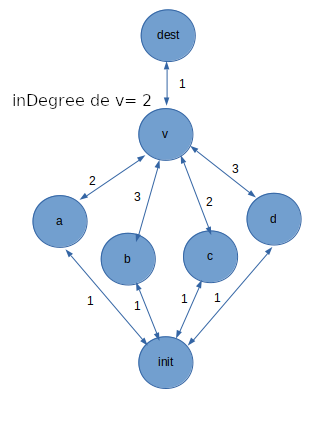
\includegraphics[width=0.9\linewidth]{Figura1}
		\caption{Ejemplo de cálculo del $inDegree$ del vértice v con respecto a $init$ y $dest$.}
		\label{fig:figura1}
	\end{figure}
	
	
	\begin{description}
		\item[Demostración] Se demostrará que todas la aristas que participan en algún camino de costo mínimo están siendo contadas una sola vez (1) y que si alguna se cuenta, es necesariamente porque participa en un camino de costo mínimo(2).\\
		
		(1) $\Rightarrow$\\
		Se tiene a $s$ y $t$, nodos inical y destino. Para cualquier arista $a$ = $<u, v>$ que pertenece a algún camino de costo mínimo entre $s$ y $t$. Esta arista sólo puede ser contada durante el análisis de $u$ y $v$, pues sólo se cuentan aristas adyacentes a los nodos, y ella es sólo adyacente a estos dos. Como pertenece a un camino de costo mínimo $c$ entre $s$ y $t$, y las aristas no pueden tener costo <= 0 (porque las carreteras no pueden tener longitud 0) entonces $u$ y $v$ participan en algún camino de costo mínimo y por tanto estos nodos serán analizados.\\
		
		\begin{description}
			\item[Lema 1] si a = $<u, v>$ participa en algún camino de costo mínimo $c$ de $s$ a $t$, entonces participa en un camino de costo mínimo de $s$ a $u$ o a $v$.
		\end{description}
		
		\begin{description}
			\item[Demostración] suponiendo sin pérdida de generalidad que $a$ aparece en un camino de costo mínimo de $s$ a $t$, saliendo de $u$ y entrando en $v$, entonces a tiene que pertenecer a un camino de costo mínimo de $s$ a $v$, pues de lo contrario existiría una forma de llegar de $s$ a $v$ con menor costo de lo que llevaba $c$ al llegar a $v$ y al unir esta forma con la forma de llegar de $v$ a $t$ en $c$, se obtendría un camino con costo menor que el mínimo.
		\end{description}
		
		Se dirá, sin pérdida de generalidad que a aparece en un camino de costo mínimo de $s$ a $v$, por tanto no podrá aparecer en uno de $s$ a $u$.
		
		\begin{description}
			\item[Lema 2:] sea a = $<u, v>$, de costo $c$ > 0, si a aparece en un camino de costo mínimo de un nodo $s$ a $v$, no podrá aparecer en uno de $s$ a $u$.
		\end{description}
		
		\begin{description}
			\item[Demostración:] sea $cst_u$, $cst_v$ el costo de ir de $s$ a $u$ y de $s$ a $v$ respectivamente. Como a participa en un camino de costo mínimo de $s$ a $v$, entonces \\
			$$cst_v = cst_u + c$$
			$$\Rightarrow c = cst_v - cst_u$$
			Suponiendo que a participara en un camino de costo mínimo de s a u, entonces:\\
			$$cst_u = cst_v + c$$
			$$\Rightarrow c = cst_u – cst_v$$
			$$\Rightarrow cst_u - cst_v = cst_v - cst_u = c$$
			$$\Rightarrow c = 0$$
		\end{description} 	
		
		
		Luego, como sólo participa en un camino de costo mínimo de $s$ a $v$, sólo será contada en el análisis de $v$ y no en el de $u$. Como el análisis de $v$ depende sólo de la existencia de un camino de costo mínimo y no se analiza nuevamente a pesar de que existan varios, entonces v será analizado sólo una vez y en este análisis se contará a a sólo una vez, ya que contar o no a a también depende de la existencia de un camino de costo mínimo en el que participe y no de en cuántos participe. Luego a será contada por $v$, y sólo por $v$, una sola vez.\\
		
		(2) $\Rightarrow$ \\
		La única forma en que el análisis cuenta aristas es cuando analiza un vértice adyacente a esta y se percata de que esta pertenece a algún camino de costo mínimo de s a una de sus puntas, digamos v, que pertenece a un camino de costo mínimo de $s$ a $t$. Como a pertenece a un camino mínimo de $s$ a $v$ y $v$ pertenece a uno de $s$ a $t$, entonces a pertenece a uno de $s$ a $t$, pues de lo contrario existiría una forma de llegar a $t$, pasando por $v$, con costo menor que el de la menor forma de llegar de $s$ a $v$, unida a la mejor forma de llegar de $v$ a $t$, lo que no es posible.\\
	\end{description}

	
	
	
	Una vez demostrado que analizando el problema de esta forma se cuentan correctamente todos los casos del problema, sólo resta mostrar que el algoritmo implementado hace, efectivamente, este análisis. Las distancias calculadas con el algoritmo \texttt{\ttfamily floyd-Warshall} son almacenadas en la lista distances. Luego se construye la matriz \texttt{\ttfamily inEdges}, que, en la posición $s$, $v$ tendrá la cantidad de aristas pertenecientes a $v$, que pertenecen a algún camino de costo mínimo entre $s$ y $v$. Para rellenar esta lista se tomarán todos los pares de vértices conectados $u$, $v$ y el costo de sus aristas correspondientes \texttt{\ttfamily cst}; luego se toma a cada vértice $k$ de $G$ y:\\
	- Si la distnacia mínima de $k$ a $u$ sumada con \texttt{\ttfamily cst} es igual a la distancia mínima de $k$ a $v$, entonces la arista $<u,v>$ forma parte de un camino de costo mínimo de $k$ a $v$ y por tanto \texttt{\ttfamily inEdges} en $k$, $v$ es incrementado en 1.\\
	- Si la distnacia mínima de $k$ a $v$ sumada con \texttt{\ttfamily cst} es igual a la distancia mínima de $k$ a $u$, entonces la arista $<u,v>$ forma parte de un camino de costo mínimo de $k$ a $u$ y por tanto \texttt{\ttfamily inEdges} en $k, u$ es incrementado en 1.\\
	Para retornar basta con tomar nuevamente cada par de vértices $u$, $v$ (ordenados de la forma apropiada para la respuesta) y analizar para cada vértice $k$ del grafo, si $k$ pertenece a algún camino de costo mínimo de $u$ a $v$, o lo que es igual, si la distancia mínima de $u$ a $k$, más la distancia mínima de $k$ a $v$ es igual a la distancia mínima de $u$ a $v$. En caso positivo, al resultado $c_{uv}$ que se está calculando se le adiciona \texttt{\ttfamily inEdges} en $u$,$k$.\\
	
	El algoritmo cuenta con una ejecución de \texttt{\ttfamily floyd-warshall} de costo $n^3$ y dos ciclos $for$ que hacen siempre a lo sumo $n^3$ iteraciones pues pasan por todas las parejas de vértices y dadas estas, por cada vértice del grafo. Luego el costo temporal del algoritmo pertenece a $O(n^3)$.\\
%-----------------------------------------------------------------------------------
\label{end}

\end{document}

%===================================================================================
